\documentclass[12pt,a4paper,fleqn]{bv_report}


\usepackage{latexsym}
\usepackage{amsmath}
%\usepackage{amssymb}
\usepackage{gensymb}
\usepackage{graphicx}
\graphicspath{{Pictures/}}
\usepackage{subfig}
\usepackage[skip=0pt]{caption}
\usepackage{float}
\usepackage{calc,ifthen,xspace}
%\usepackage{colortbl}
%\usepackage{color}
%\usepackage{xcolor}
\usepackage{fancyhdr}
%\usepackage{bbding}
%\usepackage{wasysym}
\usepackage{hyperref}
%
%\hypersetup{colorlinks, citecolor=black, filecolor=black,  linkcolor=black,  urlcolor=blue}


\usepackage{listings}             % Include the listings-package
\lstdefinestyle{customc}{
  belowcaptionskip=1\baselineskip,
  breaklines=true,
  frame=L,
  xleftmargin=\parindent,
  language=C,
  showstringspaces=false,
  basicstyle=\footnotesize\ttfamily,
  keywordstyle=\bfseries\color{green},
  commentstyle=\itshape\color{purple},
%  commentstyle=\itshape\color{red},
  identifierstyle=\color{blue},
  stringstyle=\color{orange},
}
\lstset{language=C++,style=customc}          % Set your language (you can change the language for each code-block optionally)
\newcommand{\includecode}[2][c]{\lstinputlisting[caption=#2, escapechar=, style=customc]{#2}<!---->}



%For flowcharts
\usepackage[latin1]{inputenc}
\usepackage{color}
\usepackage{tikz}
\usetikzlibrary{shapes,angles,arrows,arrows.meta,calc,intersections,patterns}
\usepackage{pgfplots}
\usepgfplotslibrary{fillbetween}
\usepackage{tkz-graph}
%%%%%%%%%%%

\usepackage{bm}

\setlength{\parindent}{0.0cm}
\setlength{\parskip}{0.4cm plus3mm minus3mm}

\def\pm{\ ^+_- \ }
\def\mp{\ ^-_+ \ }

\setlength{\oddsidemargin}{0.00cm}
\setlength{\topmargin}{-0.50cm}
\setlength{\textwidth} {16.00cm}
\setlength{\textheight}{23.20cm}



\titrerapport{User guide of foamStar}
\nomaffaire{OpenFOAM}
\noata{ATA 1350A}
\nont{NT 3259}
\reva{0}\datea{March 17th 2017}\writtenbya{Charles Monroy}\objreva{}\checkedbya{}
%\marineconditions


\begin{document}

%\let\start@align@nopar\start@align

\bvpage

\tableofcontents

\clearpage

%\input{macro}

\input{introduction}

\chapter{Installation}


\section{Mandatory packages for foamStar}

It is necessary to install Lapack on the platform.
\begin{lstlisting}[language=bash]
  $ sudo apt-get install liblapack-dev liblapack-doc-man liblapack-doc liblapack-pic liblapack3 liblapack-test liblapack3gf liblapacke liblapacke-dev
\end{lstlisting}


\chapter{Automatic generation of a mesh for sea-keeping}
\label{mesh}

The CFD mesh for sea-keeping can be generated by several methods. The most common uses standard OpenFoam tools such as \emph{snappyHexMesh} but STAR-CCM+ mesh generator can be used for tricky geometries.

\section{Body geometry}

Geometry of the body (ship) must be handled with care. Since most finite element meshes doesn't provide fine enough description of the hull, it is advised to start directly from the hull geometry (IGES file or other).

CFD meshing tools require a geometry in stereolithography format (.stl), this file can be created using standard meshing software such as FEMAP or Gmsh. Please note that STL geometry must particularly be refined in curved areas such as bow and stern parts in order to precisely represent actual hull geometry. IGES and STL samples are presented in Fig. \ref{geom}.

\begin{figure}[htbp]
\begin{center}
\subfloat[Geometries in IGES (top) and STL (bottom) formats]{
\includegraphics[width=8.5cm]{igs_stl.png}
\label{geom1}
}
\subfloat[STL refinement in bow area]{
\includegraphics[width=8.5cm]{fine_stl.png}
\label{geom2}
}
\end{center}
\caption{Body geometry}
\label{geom} 
\end{figure}

\section{CFD mesh generation (fsMesher)}

A python script has been developed for convenient CFD mesh generation with OpenFoam tools,  it can be found in \emph{foamBazar} repository. This script works with an input file described hereafter.

\subsection{fsMesher input file}

Input file for fsMesher python script contains all information needed for automatic CFD mesh generation, the corresponding extension is .cfg. A template can automatically be created using the following command:
\begin{lstlisting}[language=bash]
$ fsMesher.py -p
\end{lstlisting}

Input file options are described hereafter:
\paragraph{STL geometry file}
Multiple non-overlapping STL geometry files can be used to define the body. A specific patch will be created for each STL file. At least one file must be defined:
\begin{lstlisting}[language=bash]
# STL geometry files
stlFile0 = ./body.stl
stlFile1 = ./deck.stl
stlFile2 = ./stern.stl
\end{lstlisting}

\paragraph{Refinement in areas with strong curvature}
Areas with strong curvature such as bow and stern parts can be specified in order to be refined automatically. User must provide these areas in STL format.
\begin{lstlisting}[language=bash]
# Extra refinement in bow/stern areas with strong curvatures
refineSurf = kcs-curves.stl
\end{lstlisting}

\paragraph{Draft}
Draft must be defined from keel in the STL file coordinates system. It can be set to "None" if the geometry is already in correct position, otherwise the geometry will be moved relatively to free surface.
\begin{lstlisting}[language=bash]
# Draft (measured from keel)
draft = 15.0
\end{lstlisting}

\paragraph{Heading}
Heading is defined in degrees by the following parameter, 180\degree  corresponds to head sea. If heading is different from head or following sea, symmetric mesh can't be used.
\begin{lstlisting}[language=bash]
# Heading (in degrees)
heading = 180
\end{lstlisting}

\paragraph{Side to mesh}
In case of head or following sea, only one half of the domain has to be meshed. This parameter is used to select which side must be considered ("port" or "starboard"). In case of non-symmetrical mesh, the option "both" should be used.
\begin{lstlisting}[language=bash]
# Side : port, starboard or both ?
side = port
\end{lstlisting}

\paragraph{Domain size}
The size of the whole CFD domain is defined in relation with ship overall length (LOA). Six coefficients ($c_1$, ..., $c_6$) must be defined to set domain boundaries such as:
\begin{itemize}
\item $X_{min}= c_1 \cdot \text{LOA}$
\item $X_{max}= c_2 \cdot \text{LOA}$
\item $Y_{min}= c_3 \cdot \text{LOA}$
\item $Y_{max}= c_4 \cdot \text{LOA}$
\item $Z_{min}= c_5 \cdot \text{LOA}$
\item $Z_{max}= c_6 \cdot \text{LOA}$
\end{itemize}
Figure \ref{boundaries} shows the location of boundaries. Default values (-3.0, 2.5, -2.0, 2.0, -0.82124, 0.5555) can be used by setting the keyword to "auto".
\begin{lstlisting}[language=bash]
# Domain size relatively to LOA [X(min,max) Y(min,max) Z(min,max)]
domain = -3.0, 2.5, -2.0, 2.0, -0.82124, 0.5555
\end{lstlisting}

\begin{figure}[htbp]
\begin{center}
    \def\setA{(0,0) circle (1)}
    \def\setB{(0,0) circle (1)}
    
    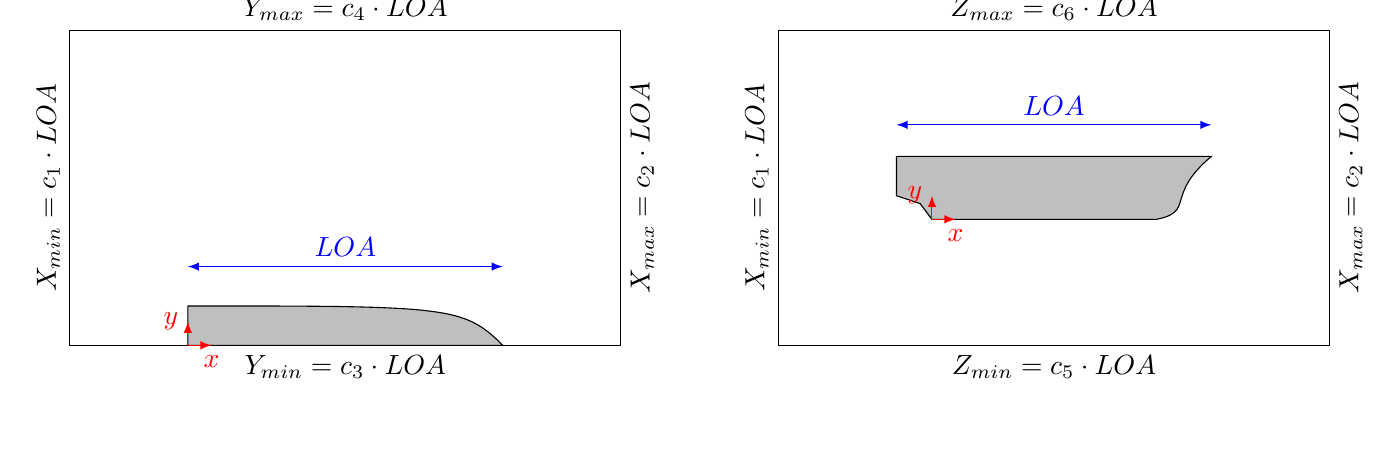
\begin{tikzpicture}
        % Top view
        \draw (-8,2) -- (-1,2) 
            node[midway,above] {$Y_{max}=c_4 \cdot LOA$}
            -- (-1,-2)
            node[midway,below,sloped,rotate=180] {$X_{max}=c_2 \cdot LOA$}
            -- (-8,-2)
            node[midway,below] {$Y_{min}=c_3 \cdot LOA $}
            -- (-8,2)
            node[midway,above,sloped] {$X_{min}=c_1 \cdot LOA$};
        \draw[fill=black!25] (-6.5,-2) -- (-6.5,-1.5) .. controls (-3.2,-1.5) and (-3,-1.5) .. (-2.5,-2) -- (-6.5,-2);
        
        \draw[latex-latex,blue] (-6.5,-1) -- (-2.5,-1) node[midway,above] {$LOA$};
        \draw[-latex,red] (-6.5,-2) -- (-6.2,-2) node[below] {$x$};
        \draw[-latex,red] (-6.5,-2) -- (-6.5,-1.7) node[left] {$y$};
        
        % Side view
        \draw (1,2) -- (8,2) 
            node[midway,above] {$Z_{max}=c_6 \cdot LOA$}
            -- (8,-2)
            node[midway,below,sloped,rotate=180] {$X_{max}=c_2 \cdot LOA$}
            -- (1,-2)
            node[midway,below] {$Z_{min}=c_5 \cdot LOA $}
            -- (1,2)
            node[midway,above,sloped] {$X_{min}=c_1 \cdot LOA$};
        \draw[fill=black!25] (5.8,-0.4) -- (2.95,-0.4) -- (2.8,-0.2) -- (2.5,-0.1) -- (2.5,0.4) -- (6.5,0.4) -- (6.5,0.4) .. controls (5.9,-0.1) and (6.3,-0.3) .. (5.8,-0.4);
        
        \draw[latex-latex,blue] (2.5,0.8) -- (6.5,0.8) node[midway,above] {$LOA$};
        \draw[-latex,red] (2.95,-0.4) -- (3.25,-0.4) node[below] {$x$};
        \draw[-latex,red] (2.95,-0.4) -- (2.95,-0.1) node[left] {$y$};
    \end{tikzpicture}
\end{center}
\caption{Definition of domain boundaries}
\label{boundaries} 
\end{figure}

\paragraph{Characteristic length}
Overall length (LOA) is usually directly computed from the geometry ("auto") but it can also be user-defined with this parameter.
\begin{lstlisting}[language=bash]
# Characteristic length
LOA = 300.
\end{lstlisting}

\paragraph{Free surface zone}
The vertical extent of the free surface refined zone is defined in relation with ship overall length (LOA). Two coefficients ($c_1$, $c_2$) must be defined to set domain boundaries such as:
\begin{itemize}
\item $Z_{min}= -c_1 \cdot \text{LOA}$
\item $Z_{max}= c_2 \cdot \text{LOA}$
\end{itemize}
Default values (0.02, 0.01) can be used by setting the keyword to "auto".
\begin{lstlisting}[language=bash]
# Free surface zone relatively to LOA [Z(min,max)]
fsZone = 0.02, 0.01
\end{lstlisting}

\begin{figure}[htbp]
\begin{center}
    \def\setA{(0,0) circle (1)}
    \def\setB{(0,0) circle (1)}
    
    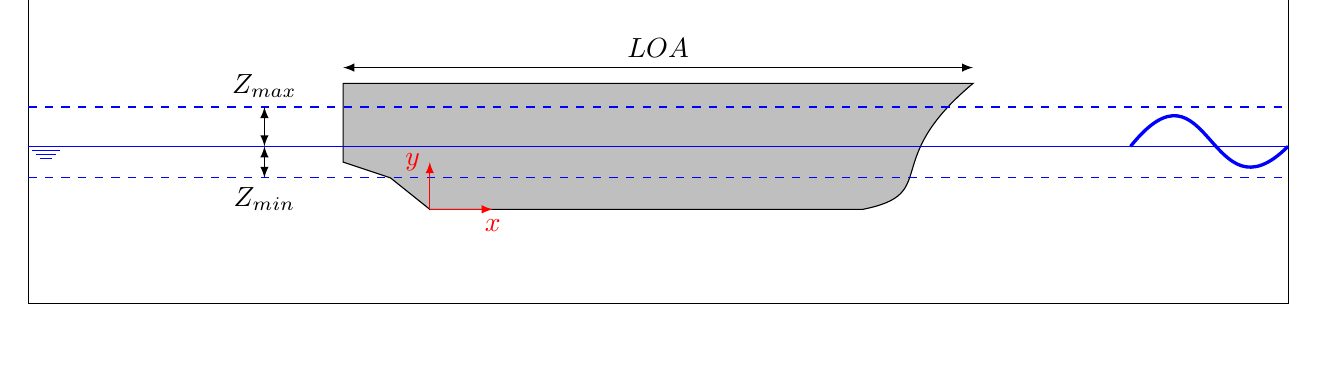
\begin{tikzpicture}        
        % Side view
        \draw (-8,2) rectangle (8,-2);
        \draw[fill=black!25] (2.6,-0.8) -- (-2.9,-0.8) -- (-3.4,-0.4) -- (-4,-0.2) -- (-4,0.8) -- (4,0.8) -- (4,0.8) .. controls (2.8,-0.2) and (3.6,-0.6) .. (2.6,-0.8);
        
        \draw[blue] (-8,0) -- (8,0);
        \draw[blue] (-7.95,-0.05) -- (-7.60,-0.05);
        \draw[blue] (-7.90,-0.10) -- (-7.65,-0.10);
        \draw[blue] (-7.85,-0.15) -- (-7.70,-0.15);
        
        \draw[blue,dashed] (-8,0.5)  -- (8,0.5);
        \draw[blue,dashed] (-8,-0.4) -- (8,-0.4);
        \draw[blue,very thick] (8,0) .. controls (7,-1) and (7,1.25) .. (6,0);
        
        \draw[latex-latex] (-5,0.0) -- (-5,0.5)  node[above] {$Z_{max}$};
        \draw[latex-latex] (-5,0.0) -- (-5,-0.4) node[below] {$Z_{min}$};
        
        \draw[latex-latex] (-4,1) -- (4,1) node[midway,above] {$LOA$};
        \draw[-latex,red] (-2.9,-0.8) -- (-2.1,-0.8) node[below] {$x$};
        \draw[-latex,red] (-2.9,-0.8) -- (-2.9,-0.2) node[left] {$y$};
    \end{tikzpicture}
\end{center}
\caption{Definition of domain boundaries}
\label{boundaries} 
\end{figure}

\paragraph{Cell height within the free surface zone}
Cell height in free surface zone can be defined with this parameter. Default value (0.33*fsZmax) can be used by setting the keyword to "auto".
\begin{lstlisting}[language=bash]
# Cell height within the free surface zone
fsCellHeight = 1.5
\end{lstlisting}

\paragraph{Cell ratio length/height within the free surface zone}
Cell ratio  length/height in free surface zone can be defined with this parameter. Default value (4) can be used by setting the keyword to "auto".
\begin{lstlisting}[language=bash]
# Cell ratio length/height within the free surface zone
fsCellRatio = 4
\end{lstlisting}

\paragraph{Type of refinement box(es) in the domain}
The type of refinement boxes can be defined with the following parameter. Available options are "wave", "kelvin" or "both".
\begin{lstlisting}[language=bash]
# Type of refinement box(es) in the domain
refBoxType = wave
\end{lstlisting}

\paragraph{Data for refinement boxes}
Refinement boxes can be defined in an automatic and manual way. The automatic way requires definition of two parameters: "refBoxData" and "refBoxRatio". The fist corresponds to the number of refinement boxes and the second to the ratio between the smallest and the largest boxes. Default values (3 for both parameters) can be used for automatic refinement by setting the keywords to "auto". Refinement boxes can also be defined manually with parameter "refBoxData" followed by the number of boxes and the corresponding coordinates in X-Y plane $X_{min}$, $X_{max}$, $Y_{min}$, $Y_{max}$ for each box.
\begin{lstlisting}[language=bash]
# Automatic definition of refinement box(es) in the domain
refBoxData = 3
refBoxRatio = 3

# Manual definition of refinement box(es) in the domain
# NbBox, Xmin1, Xmax1, Ymin1, Ymax1, Xmin2, Xmax2, Ymin2, Ymax2, ... 
refBoxData = 2, -500, 600, -50, 350, -250, 600, -50, 350 
\end{lstlisting}

\paragraph{Cell buffer between refinement level}
In order to avoid brutal refinement between each zone, a minimal number of cells can be defined between two zones. Default value (4) can be used by setting the keyword to "auto".
\begin{lstlisting}[language=bash]
# Cell buffer between refinement level
cellBuffer = 4
\end{lstlisting}

\paragraph{Additional refinement at the bow and stern regions}
Additional refinement in bow and stern areas can be defined with this parameter. Such refinements are particularly used to improve slamming accuracy in these zones. Refinement boxes size are defined by a coefficient relatively to LOA. Bow and sterm refinements can be disabled by setting these parameters to zero. Default values (0.2) can be used by setting the keyword to "auto".
\begin{lstlisting}[language=bash]
# Additional refinement at the bow region
refineBow = 0.2

# Additional refinement at the stern region
refineStern = 0.2
\end{lstlisting}

\paragraph{Additional vertical refinement in the free surface zone near the ship}
Additional vertical refinement around the free surface in the ship area can be defined with this parameter. The value can be "True" or "False".
\begin{lstlisting}[language=bash]
# Additional vert. refinement in the free surface zone near the ship
refineFS = False
\end{lstlisting}

\paragraph{Dimensions of boundary layers}
Boundary layers can be defined around the body using this parameter. Default values can be used by setting the keyword to "auto". The following values must be defined:
\begin{itemize}
\item number of layers (default=3)
\item layer growth (default=1.3)
\item thickness of final boundary layer (default=0.7)
\item minimal thickness ratio (default=0.7)
\end{itemize}
\begin{lstlisting}[language=bash]
# Dimension for boundary layers (relative to cell size)
# nLayers, layerGrowth, finalLayerThickness, minThicknessRatio
layers = 3, 1.3, 0.7, 0.7
\end{lstlisting}

\paragraph{Disable location for selected patch}
Boundary layers are created on all patches by default but can be removed from some of them is not needed (e.g. it is usually not needed on deck). The name(s) of patch(es) to be removed from boundary layer must be given (separated by commas).
\begin{lstlisting}[language=bash]
# Deactivate boundary layer on patch(es)
disableLayers = deck
\end{lstlisting}

\paragraph{Additional setting}
Follonwig additional settings can be added to input file:

\begin{lstlisting}[language=bash]
# these are optional settings for fsMesher.py
[fsMesher-control]

# these switches can be called from command line
# settings called from command line overrule settings in this config-file
# note: NPROCS has no effect when "system/decomposeParDict" exists
DEBUG = True
NPROCS = 4
EXEC_BLOCKMESH = True
EXEC_REFINEBOX = True
EXEC_REFINEPROXIMITY = True
EXEC_SNAP = True
EXEC_ADDLAYERS = True

# main stl-filename in "./constant/triSurface/"
DEFAULT_SHIP_STL = ship.stl

# Self-explained settings ... 
# log-file for foam tools is defined in CMD_keepLog.
# output from python script is flushed to stdOut
CMD_keepLog = ' >> ./log.fsMesher 2>&1 '
CMD_showLog = 'echo "\nlog-file: ./log.fsMesher"; tail -45 ./log.fsMesher; echo "Please see log-file: ./log.fsMesher"'
CMD_blockMesh = 'blockMesh'
CMD_autoPatch = 'autoPatch -overwrite 80'
CMD_setSet = 'setSet -latestTime'
CMD_refineMesh = 'refineMesh'
CMD_snappyHexMesh = 'snappyHexMesh'
CMD_decomposePar = 'decomposePar -force -latestTime'
\end{lstlisting}

\subsection{Launch fsMesher}

Before generating the CFD mesh, it can be useful to check the commands that will be executed by fsMesher script. This can be done by using "-n" option. The results can also be stored in a log file using this command :
\begin{lstlisting}[language=bash]
$ fsMesher.py -f fsMesher.cfg -n > log.dryrun
\end{lstlisting}

The script can then be executed with :
\begin{lstlisting}[language=bash]
$ fsMesher.py -f fsMesher.cfg
\end{lstlisting}

Once finished, if parallel computation has been used, one need to reconstruct the data using the following command:
\begin{lstlisting}[language=bash]
$ reconstructParMesh -latestTime
\end{lstlisting}

The resulting meshes can be found in time folders, the higher value corresponds the final mesh and others are intermediate steps. Meshes can directly be viewed with Paraview (Windows users should insert a void "*.foam" file to use with Paraview).

\begin{figure}[htbp]
\begin{center}
\includegraphics[width=12cm]{CFD_mesh.png}
\end{center}
\caption{CDF mesh with ship}
\label{cfd_mesh} 
\end{figure}


\subsection{Recommendations for mesh generation}

Here are summarized some common advise for mesh quality:
\begin{itemize}
\item Number of cell in X-direction should be at least 100 per wave length
\item Symmetry plane has to be defined on patch Y0 for head seas. It is advised to add another symmetry plane on patch Y1 for high forward speed cases
\item All body patches created by fsMesher (hull, deck, ...) should be merged into one single patch manually or using \emph{createPatch}
\end{itemize}

\chapter{Pre-computing structural information}
\label{homer}

All structural information needed for mechanical equation solving and flexible modes can be pre-computed from an Homer 2 model.

\section{Running Homer}
Once the model has been set up, HmFEM has to be run with the following body options. Please refer to Homer user guide for more information about Homer keywords.

\begin{lstlisting}[language=fortran]
# Strcutural mesh information
STRUCTURALMESH = body.dat
STRUCTURALCOORDINATES = 0. 0. -11.75 0. 0. 0.
STRUCTURALLENGTHUNIT = m
STRUCTURALMASSUNIT = kg

# Number of flexible modes if required
STRUCTURALNFLEXIBLEMODES = 3

# Enable specific outputs for OpenFoam
PREPAREOPENFOAM = 1

# Sections definition
SECTIONS
CUT   -6.00 0. 12.015 1. 0. 0.
CUT   82.83 0. 12.015 1. 0. 0.
CUT  150.78 0. 12.015 1. 0. 0.
CUT  223.23 0. 12.015 1. 0. 0.
CUT  295.00 0. 12.015 1. 0. 0.
ENDSECTIONS
\end{lstlisting}

HmFEM will then run normally and create the following files that are useful for foamStar:
\begin{itemize}
\item mesh : Finite\_Elements\_Analysis{\textbackslash}HmFEM{\textbackslash}\textbf{body\_Bulk.dat}
\item mass matrix : Finite\_Elements\_Analysis{\textbackslash}HmFEM{\textbackslash}\textbf{body\_dmig.pch}
\item mode shapes : Finite\_Elements\_Analysis{\textbackslash}HmFEM{\textbackslash}\textbf{body\_md.pch}
\item don file : User\_Outputs{\textbackslash}HmFEM{\textbackslash}\textbf{body.don}
\end{itemize}

\section{Initialize structural information for foamStar}

Structural data pre-processing for foamStar is performed using the module \emph{initFlx} together with a standard OpenFoam input file \emph{initFlxDict} described hereafter:

\begin{lstlisting}[language=C]
FEM_STRUCTURALMESH_VTU
{
    datFile "body_Bulk.dat";
    mdFile "body_md.pch"; selected (7 8 9);
    dmigMfile "body_dmig.pch";
    dmigKfile "body_dmig.pch";
    pchCoordinate (0 0 -11.75 0 0 0);
    pchScaleMode  0.25909281809220411E+05;
    pchLengthUnit 1;
    pchMassUnit   1;

    patches (ship); ySym (true);
}
\end{lstlisting}

\begin{itemize}
\item \textbf{datFile} : finite element mesh provided by Homer (*\_Bulk.dat)
\item \textbf{mdFile} : modes shapes punch file given by Homer (*\_md.pch)
\item \textbf{selected} : select flexible modes to use for simulation (starting from mode 7)
\item \textbf{dmigMfile} : mass matrix punch file provided by Homer (*\_dmig.pch)
\item \textbf{dmigKfile} : stiffness matrix punch file provided by Homer (*\_dmig.pch)
\item \textbf{pchCoordinate} : structural coordinates used in Homer
\item \textbf{pchScaleMode} : value of scaling factor of first mode in Homer
\item \textbf{pchLengthUnit} : length scaling factor to meters (m=1, mm=0.001)
\item \textbf{pchMassUnit} : mass scaling factor to kilograms (kg=1, t=1000)
\item \textbf{pchMassUnit} : mass scaling factor to kilograms (kg=1, t=1000)
\item \textbf{patches} : define patch representing the hull
\item \textbf{patches} : define if Y-symmetry is used or not
\end{itemize}

foamStar module can then be launched with the following command:
\begin{lstlisting}[language=bash]
$ initFlx
\end{lstlisting}






\chapter{Data setup}

\section{Mesh}

The mesh should be prepared in a separate folder from the calculation folder. Once created the mesh can be transferred to the calculation folder using the following command:
\begin{lstlisting}[language=bash]
$ write python template script
\end{lstlisting}




\input{logAnalyzer}

\input{ligerCluster}
%\input{equations}


%\input{logicalSchemes}

%\input{flowSolver}

%\input{sixDofMechanicalSolver}

%\input{modalMechanicalSolver}


%\chapter{Mesh computation}

%\input{FSIinteractions}


%\input{schemes}


%\input{postProcessing}

%\bibliographystyle{plain}

%\bibliography{foamStar_biblio}


\end{document}